\chapter{Adatok gyűjtése a mesterséges intelligencia betanításához}
\thispagestyle{fancy}
\pagestyle{fancy}

\section{Tervezés}
A mesterséges intelligencia hatékony betanításához elengedhetetlen, hogy a lehető legtöbb információt gyűjtsük össze egy adott játékmenet során.

\subsection{Az adatszerkezet}
Egy adott játékfolyamat az alábbi lépésekből áll:

\begin{itemize}
\item A játékos a korábbi ismeretei alapján kiválasztja, melyik sor és melyik oszlop kártyáját fordítja fel.
\item A kártya felfordítása után a játékos megtudja, milyen betű található a kártyán.
\item Az így megszerzett információ és a korábbi tudása alapján a játékos kiválasztja a következő kártyát a táblán. Itt két lehetősége van:
\begin{itemize}
\item A játékos tudja, vagy nagy valószínűséggel sejti, melyik kártya a párja az előzőnek.
\item A játékos nem tudja, vagy kis valószínűséggel sejti, hol található a párja, ezért olyan kártyát fordít fel, amiről még nincs információja, azaz felfedezi a pályát.
\end{itemize}
\item Ha a felfordított kártyák párt alkotnak, azok eltűnnek a tábláról.
\item A játékos ezt a folyamatot addig ismétli, amíg az összes kártya el nem tűnik a tábláról.
\end{itemize}

A játék teljes megértéséhez és a mesterséges intelligencia betanításához az alábbi adatokra van szükségünk:

\begin{itemize}
\item A táblán található kártyák száma. Mivel mindig egy $N \cdot N$ négyzetet használunk, ezt az értéket fixen ismerjük.
\item A leosztásban szereplő betűk.
\item A kártyafordítások sorrendje: melyik sor és oszlop kártyái lettek felfordítva, valamint mi szerepelt a memória kártyán.
\end{itemize}

A következő adatszerkezetet használtam: 

\begin{figure}[h]
\centering
 \begin{lstlisting}
{
  "data": { 
    "id": "Xx12345"
    "played_games": {
      "6": [
        {
          "card_labels": ['A','B','C','D','E','F'], 
          "card_pair_number": 6,
          "card_selections": [ 
            {
              "chosen_first": true,
              "label": "A",
              "x": 0,
              "y": 0
            },
            {
                ...
            },
          ]
        },
        {
            ...
        }
      ]
    }
  }
}
\end{lstlisting}
\caption{Tanításhoz felhasznált adatszerkezet}
\label{saveJson}
\end{figure}


A \ref{saveJson} ábra magyarázata a következő:
\begin{description}
    \item[azonosító (id)] A játékos ID-je melyet megkap a játék elindításakor. 
    \item[Played\_games] Játszott játékok, ahol a kulcs a kártyapárok száma.
    \item[6\:] Egy tömb, amely az adott kártyaszámú játékokat tartalmazza.
    \item[card\_labels\:] A kártyák lehetséges címkéi. Ezek száma megegyezik a \lstinline{card_pair_number} értékével.
    \item[card\_pair\_number\:] A kártyapárok száma, amely megegyezik a tömb kulcsával. Az adatok könnyebb kezelése érdekében ez az érték duplikálva van.
    \item[card\_selections\:] Az összes kártyahúzás a játék során, ez a tömb a játék előrehaladtával bővül.
    \item[chosen\_first\:] Megjelöli, hogy a kártyát elsőként választották-e. Ez az információ a kártyaválasztások párosságából kiszámítható.
    \item[label\:] A kártyán szereplő betű.
    \item[X,Y\:] A kártya sor- és oszlopkoordinátái.
\end{description}
\subsection{Játék előkészítése}
A tervek szerint a játékot a lehető legtöbb emberhez akartam eljuttatni, ezért a legkézenfekvőbb megoldásnak a HTML5-be történő exportálást láttam \cite{Exportin97:online}. Ehhez néhány vizuális módosítást kellett végrehajtanom.
Két fő lehetőségem volt, amelyekkel komolyabban foglalkoztam:
\begin{enumerate}
    \item  Játék és HTML sablon átalakítása: A játékot és a hozzá tartozó HTML sablont átírni úgy, hogy a weboldal JavaScriptje segítségével a JSON fájlt lementsem, amit aztán valamilyen online felületen keresztül el tudnak küldeni nekem.
    \item	Fájl szerver létrehozása: Készítek egy fájl szervert, ahova a JSON-t minden sikeres játék után elküldöm egy HTTP-kérés formájában.

\end{enumerate}


Átgondolva a lehetőségeimet, a fájl szerver mellett döntöttem, mivel így az összes tesztadat biztosan és automatikusan eljut hozzám.

A játékhoz készítettem egy \lstinline{http_client.gd} szkriptet, amelynek egyetlen feladata egy \lstinline{HTTP POST} kérés elküldése egy weboldalnak. A HTTP-kérés törzsében helyeztem el a JSON fájlt. Ezt a szkriptet minden játék befejezése után aktiváltam.

Annak érdekében, hogy a kérés mindig sikeres legyen, biztosítanom kellett, 
hogy ha egy játékosnak nincs ID-je és a beviteli mezőt üresen hagyta, akkor egy véletlenszerűen generált ID-t kapjon. 
Az ID-t a menü oldalon jelenítettem meg, és másolhatóvá tettem.
A játék állását, vagyis azt, hogy melyik játékkal mennyit játszott a játékos, a Godot automatikusan a böngésző lokális IndexedDB-jébe \cite{Exportin97:online} mentette.

Az IndexedDB \cite{UsingInd44:online} egy böngésző alapú adatbázis, amely lehetővé teszi nagy mennyiségű strukturált adat tárolását, beleértve fájlokat és bináris adatokat is. Ez egy NoSQL adatbázis, ami azt jelenti, hogy kulcs-érték párokkal dolgozik, nem pedig táblázatokkal, mint egy relációs adatbázis. 
Az IndexedDB segítségével a memoriajáték elmenti az adatait a böngészőbe, így később hozzáférhet és láthatja a játékos, hogy melyik nehézségi szinten mennyit játszott a játékkal.

Így, ha egy játékos akkor játszik, amikor a szerver nem elérhető, később is el tudja küldeni a játszott játékainak statisztikáját.\begin{figure}[h]
    \centering
    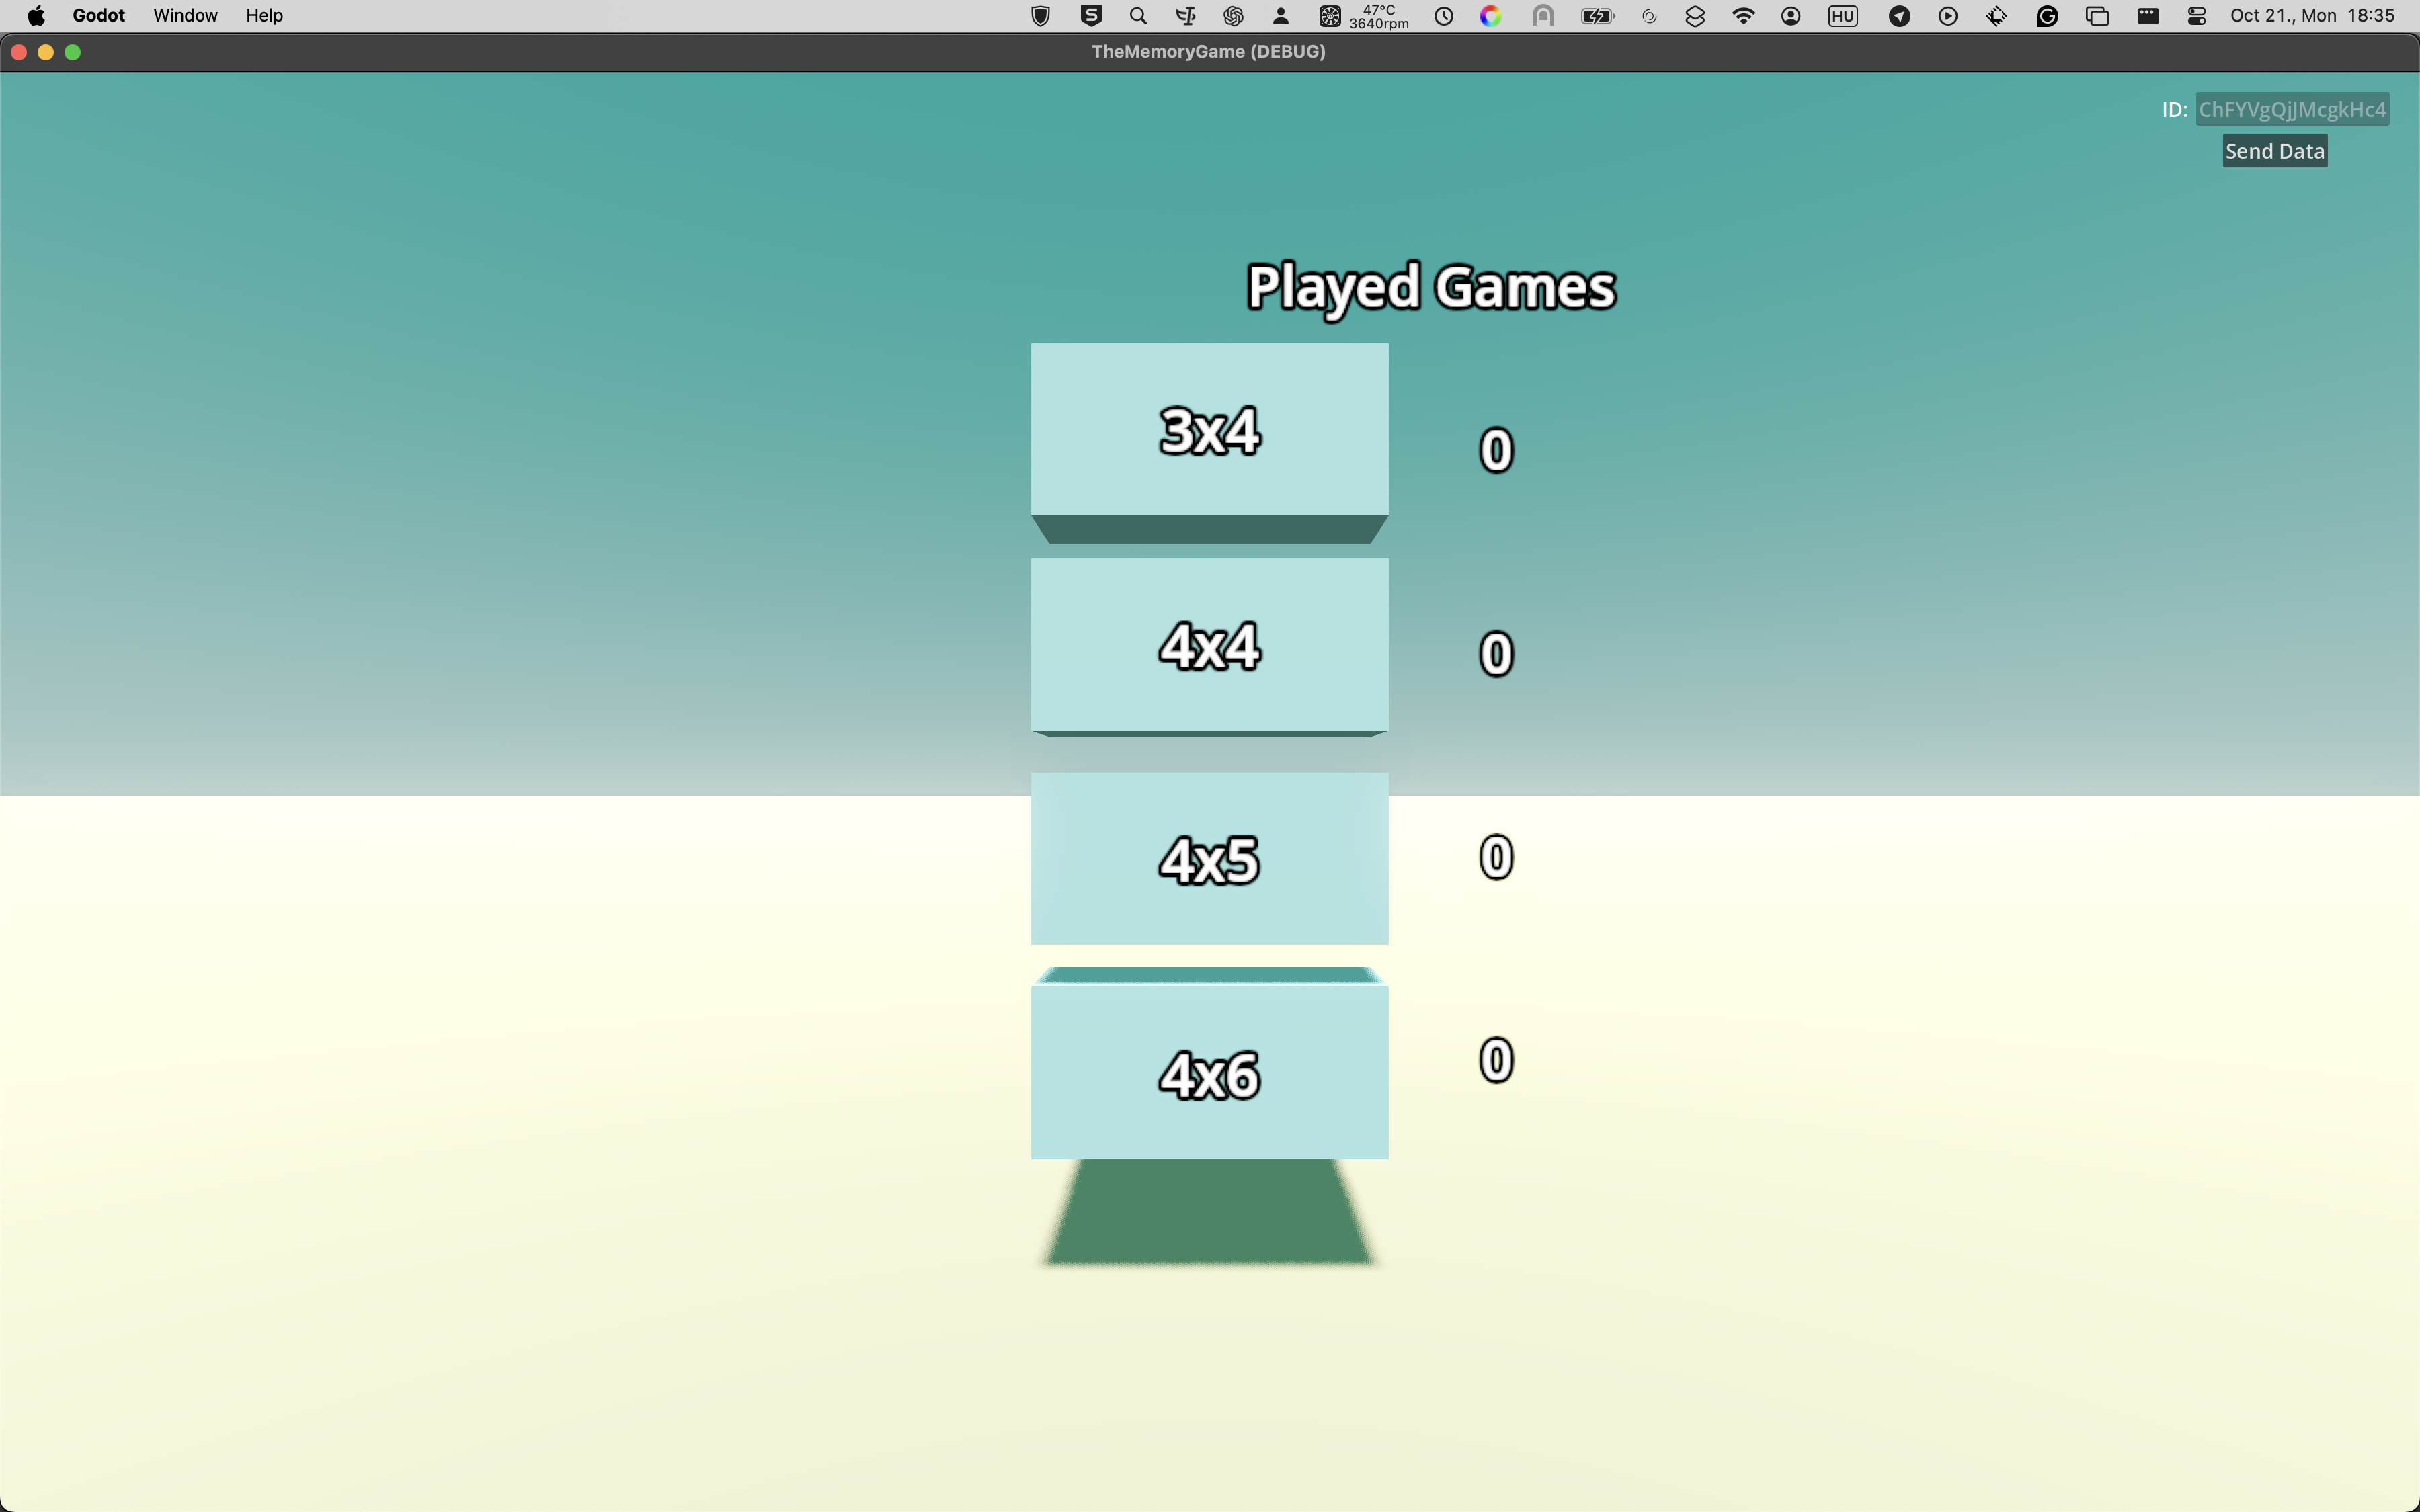
\includegraphics[width=0.75\textwidth]{img/menu_remake.png}
    \caption{Az átlakaított menü: másolható ID mező, és egy küldés gomb}
    \label{img:menu_remake}  
\end{figure}

\subsection{Játék feltöltése itch.io-ra}

A kész játékot exportáltam HTML5 formátumba, majd regisztráltam az itch.io oldalán.
Itt létrehoztam egy weboldalt a játékomnak, és elhelyeztem rajta egy rövidke leírást angolul.

A játékot elérhetővé tettem \url{https://csetom.itch.io/the-memory-game} címen (\ref{img:itch.io}. ábra). 

A beállítottam, hogy a "Run game" gombra kattintva a játék "teljes képernyős" üzemmódban induljon el, hogy kitöltse a teljes weboldalt. 

\begin{figure}[h]
  \centering
  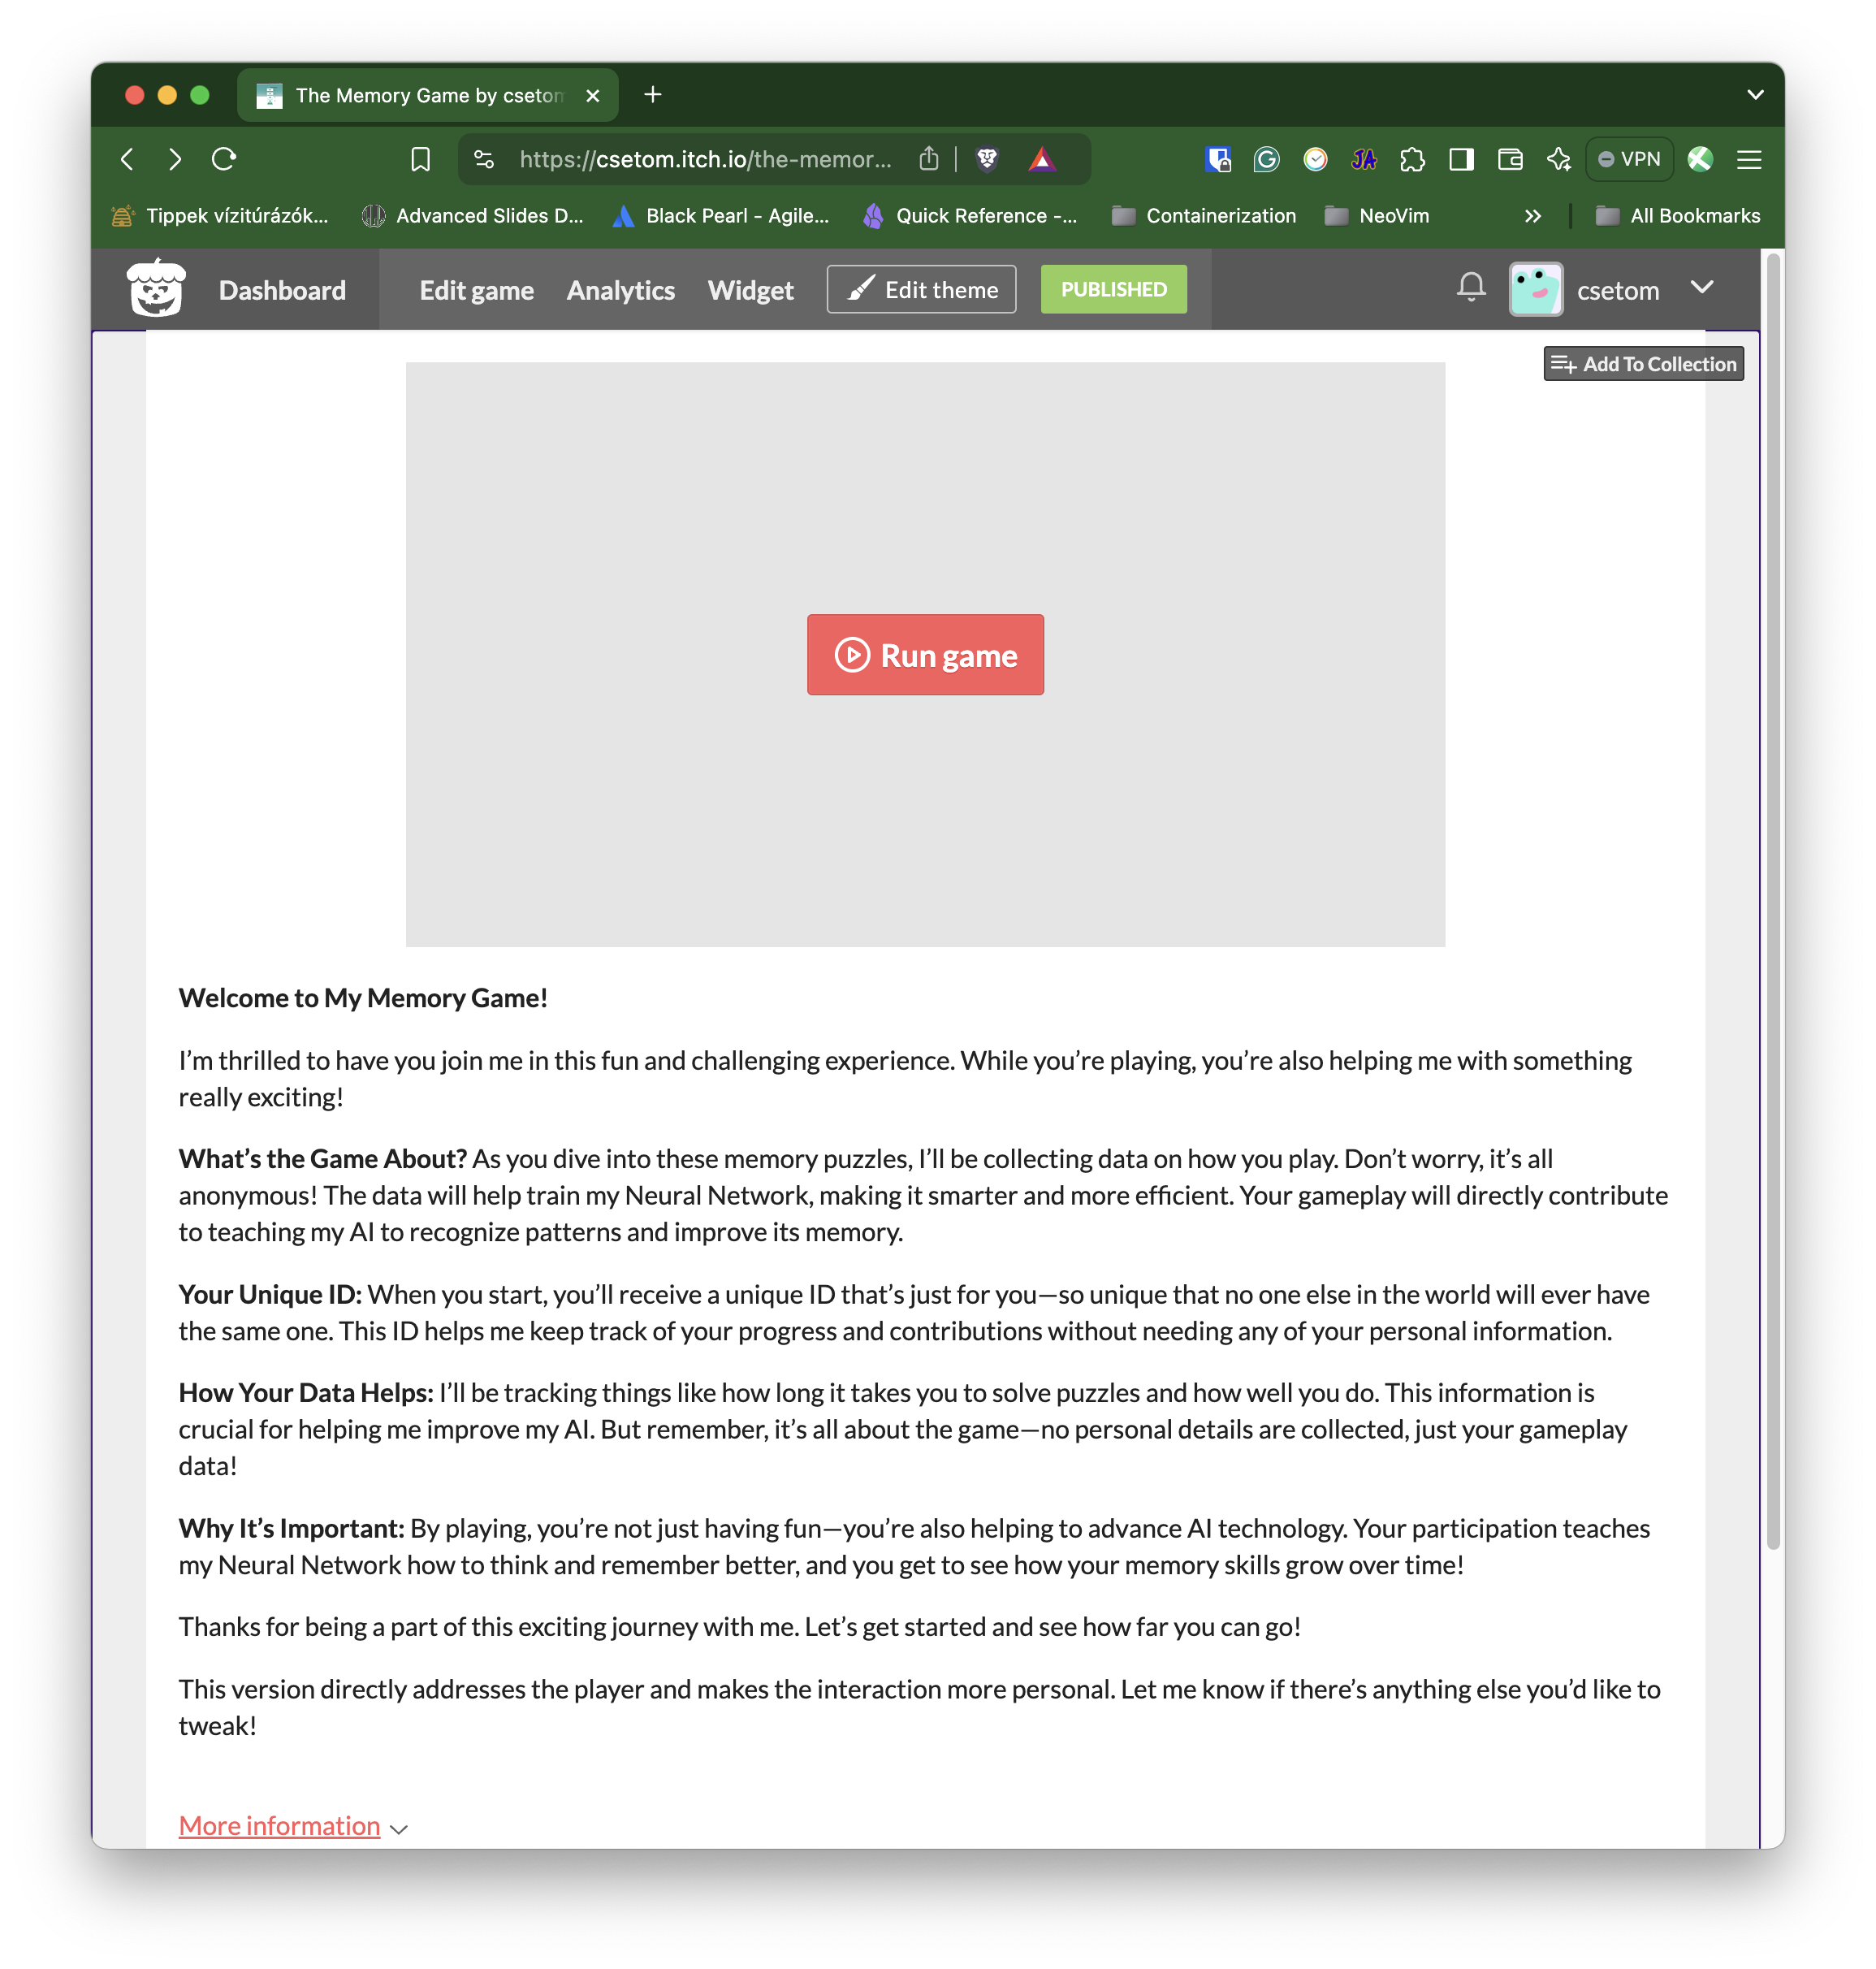
\includegraphics[width=0.75\textwidth]{img/Itch.io.png}
  \caption{Memóriajátékom itch.io oldala, ahonnan egy kattintásra futtatható a játék}
  \label{img:itch.io}  
\end{figure}


\section{Fájl szerver megvalósítása}
A fájlszerver megvalósításához JavaScriptet és Node.js-t használtam.
A szerver működtetésére az Express web framework-öt \cite{ExpressN40:online} vettem igénybe, 
A fájlszerver egyetlen végpontot biztosított, amely a \lstinline{/save_json} útvonalon volt elérhető. 
Ez a végpont fogadta az érkező JSON formátumú adatokat. A szerver feladata volt ezeknek az adatoknak a fájlrendszerbe történő mentése. 
A mentési folyamat során az adatok az ID szerint kerültek elhelyezésre külön mappákba, ahol a mappa neve a játékos ID-ja volt. 
Az egyes mappákban az aktuális időpont szerint elnevezett JSON fájlok kerültek tárolásra, például: \texttt{2023-10-21T12:34:56.json}. 
Ez a struktúra biztosította az adatok könnyű visszakereshetőségét és rendszerezhetőségét.

Annak érdekében, hogy a szerver domain néven keresztül is elérhető legyen, a Cloudflare Tunnel \cite{TunnelZe60:online} szolgáltatást alkalmaztam. 

A rendszer kényelmes használata és virtuális gépen történő telepítése érdekében a szervert és a Cloudflare-t is \cite{WhyCloud84:online} külön-külön Docker \cite{DockerAc99:online} konténerben futtattam.
A konténerek használata egyszerűvé teszi a telepítést és a menedzselést, mivel az alkalmazások és azok függőségei elszigetelten futnak. 
A Docker Compose \cite{DockerCo66:online} segítségével pedig könnyedén integrálhattam és menedzselhettem a többkonténeres alkalmazásokat, ami lehetővé tette a szerver és a Cloudflare Tunnel együttes futtatását és összehangolt működését.

\begin{figure}[h]
    \centering
\begin{lstlisting}
services:
file-server:
  build:
    context: .
  volumes:
    - ./data:/app/data
cloudflair:
  image: cloudflare/cloudflared:latest 
  command: tunnel --no-autoupdate run --token <token>
\end{lstlisting}
\caption*{docker-compose.yaml}
\label{code:docker-compose}
\end{figure}
\begin{figure}[h]
    \centering
    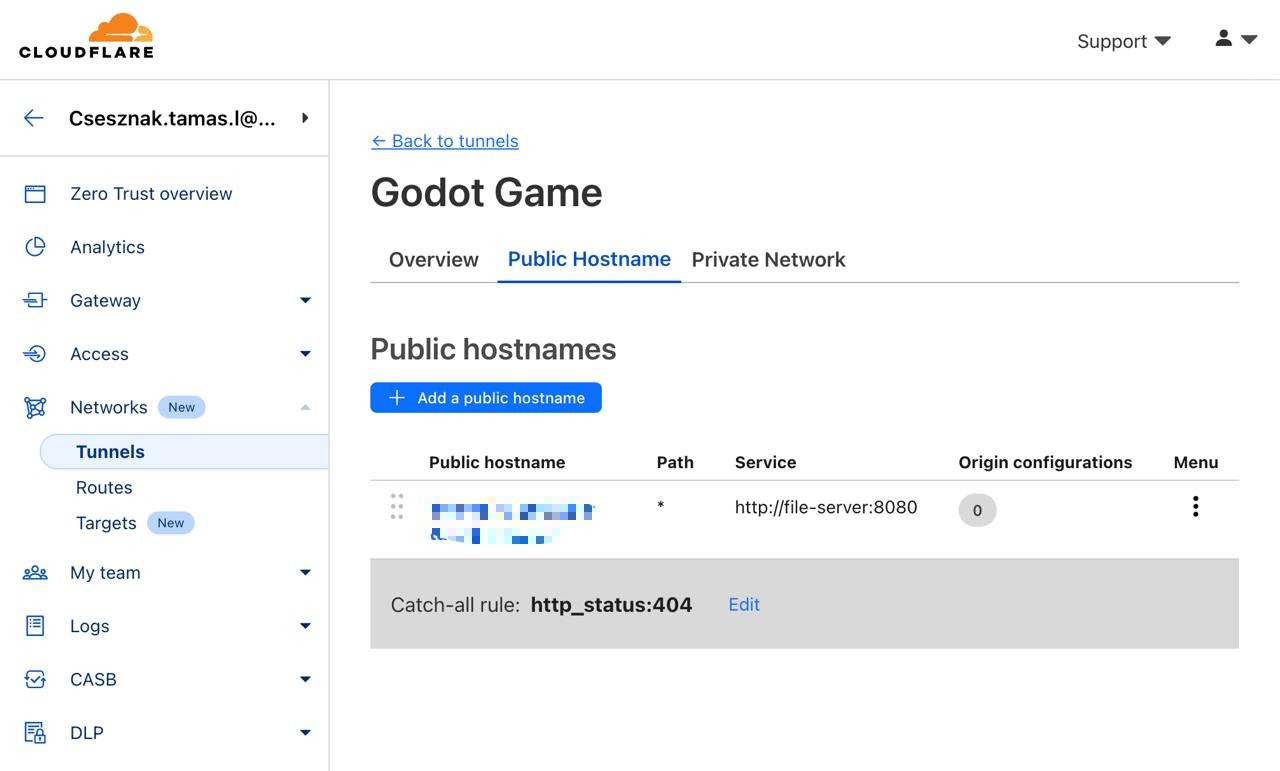
\includegraphics[width=0.75\textwidth]{img/cloudflair-censored.jpg}
    \caption{Cloudflair Tunnel konfiguráció}
    \label{img:cloudflair-config}  
\end{figure}


\subsection{Oracle Cloud}
A fájlszerver telepítéséhez először az Oracle VM-et \cite{CloudInf58:online} szerettem volna használni. Az Oracle VM egy rendkívül megbízható és skálázható megoldás, amely lehetővé teszi, hogy virtuális gépeket hozzunk létre és futtassunk különböző platformokon. Az Oracle VM számos előnnyel rendelkezik, mint például a magas teljesítmény, a robusztus biztonsági funkciók, és a kiváló támogatás. Ezen kívül számos operációs rendszerrel kompatibilis, ami megkönnyíti a különféle alkalmazások és szolgáltatások telepítését és futtatását.

Az Oracle VM-en keresztül kívántam a fájlszerveremet üzemeltetni, mivel reméltem, hogy a szolgáltatás rugalmassága és skálázhatósága előnyös lesz a projekt szempontjából. Az Oracle VM felületén könnyedén konfigurálhatók a virtuális gépek, és a hálózati beállítások is egyszerűen kezelhetők. Emellett a szolgáltatás integrálhatósága más Oracle termékekkel és szolgáltatásokkal további előnyöket kínál.

Azonban, amikor megpróbáltam igénybe venni az Oracle VM ingyenes erőforrásait, sajnálatos módon azt tapasztaltam, hogy ezek nem voltak elérhetők. 
Az ingyenes erőforrások hiánya miatt kénytelen voltam alternatív megoldást keresni.
 Ez komoly csalódást okozott, mivel úgy gondoltam, hogy az Oracle VM ideális lenne a fájlszerverem futtatására.


\subsection{Fly.io}
Miután az Oracle VM nem bizonyult járható útnak, úgy döntöttem, hogy kipróbálom a Fly.io \cite{Deployap0:online} szolgáltatását.
A Fly.io egy modern felhőalapú platform, amely lehetővé teszi az alkalmazások globális szinten történő futtatását és skálázását.
A szolgáltatás fő célja, hogy az alkalmazásokat közelebb hozza a felhasználókhoz, ezáltal csökkentve a késleltetést és javítva a teljesítményt.
A Fly.io platformja rendkívül egyszerűen használható, és számos automatizált funkcióval rendelkezik, amelyek megkönnyítik az alkalmazások telepítését és kezelését.

A Fly.io honlapja első ránézésre ígéretesnek tűnt, és úgy tűnt, hogy ingyenes használati lehetőséget is kínál.
Ez különösen vonzó volt számomra, mivel szerettem volna minimalizálni a költségeket a projekt korai szakaszában.
A Fly.io segítségével könnyedén létrehozhattam és kezelhettem a fájlszerveremet, és a platform egyszerűsége miatt gyorsan és hatékonyan tudtam dolgozni.

Azonban, amikor elkezdtem a fájlszerver telepítését és konfigurálását a Fly.io platformján, kiderült, hogy a szolgáltatás nem teljesen ingyenes.
A Fly.io használatával kapcsolatos üzenetváltások darabszámára vonatkozó díjak jelentősen 
megnövelték volna a költségeket. Ez komoly kihívást jelentett, és nem számítottam ilyen jellegű kiadásokra. 
Az ingyenesnek tűnő szolgáltatásról kiderült, 
hogy valójában nem az. Csalódtam, és ismét arra kényszerűltem, hogy más megoldásokat keressek a fájlszerverem üzemeltetéséhez.

Mindkét esetben a szolgáltatások ígéretes lehetőségeket kínáltak, de végül nem feleltek meg az elvárásaimnak az ingyenes erőforrások hiánya és a rejtett költségek miatt. Azonban a tapasztalatok segítettek abban, hogy jobban megértsem a különböző felhőalapú platformok működését és költségstruktúráját, ami hasznos lesz a jövőbeni projektek tervezésénél és megvalósításánál.
\section{Végleges megoldás}
Mivel sajnos nem találtam más alternatívát, ami ingyenes lenne, így kénytelen voltam a helyi gépemen futtatni a docker containereket, és megkérni a játék tesztelőket, hogy akkor futtassák a játékot, amikor éppen üzemel a file szerver. A tesztelőknek elküldtem az itch.io weboldalt, így nem volt szükséges számukra, hogy telepítsék a saját számítógépükre az alkamazást.

Összesen tíz embertől sikerült megfelelő mennyiségű adatot szereznem,melynek segítségével tanítottam be a mesterséges intelligenciát.